\documentclass{TDP003mall}
\usepackage[utf8]{inputenc}
\usepackage[swedish]{babel}


\newcommand{\version}{Version 1.0}
\author{Daniel Huber, \url{danhu849@liu.se}\\
  Jens Öhnell, \url{jenoh242@liu.se}}
\title{Systemdokumentation}
\date{2020-10-15}
\rhead{Daniel Huber\\
Jens Öhnell}



\begin{document}
\projectpage
\section{Revisionshistorik}
\begin{table}[!h]
\begin{tabularx}{\linewidth}{|l|X|l|}
\hline
Ver. & Revisionsbeskrivning & Datum \\\hline
1.0 & Systemdokumentation för Portfolio TDP003 & 151020 \\\hline
\end{tabularx}
\end{table}


\section{Översiktsbild}
Hemsidans syfte är att presentera information om hemsidans ägare, och presentera projekt som denna har gjort på ett sökbart sätt. Hemsidan byggs upp av ett datalager samt ett presentationslager.

\subsection{Datalagret}
Datalagrets syfte är att gör information om olika projekt åtkommlig och sökbar. Det är skrivet i Python 3, och söker mot en json-fil.

\subsection{Presentationslagret}
Presentationslagrets syfte är att göra informationen tillgänglig till slutanvändaren på ett enkelt och intuitivt sätt. Det är skrivet i Python 3 med ramverket Flask samt templatemotorn Jinja2.

\section{Specifikation - Presentationslagret}
Skapandet av hemsidan har utgått från en kravspecifikation. Denna har varit vägledande i vilken funktionalitet sidan skall ha. Den fulla specifikationen kan hittas i dokumentet \textit{Systemspecifikation av portfoliosystem}.

Sammanfattningsvis skall dock följande ingå i hemsidan:
\begin{itemize}
    \item En förstasida med bilder.
    \item En söksida som gör det möjligt att söka och sortera på diverse fält för projekten.
    \item En tekniksida som gör det möjligt att sortera projekt på använda tekniker.
    \item Bilder, både "thumbnails" och fullstora, för all projekt.
    \item Begripliga felmedelanden.
    \item Korrekta statuskoder.
\end{itemize}

\newpage
\section{Sekvensdiagram - Sökning}

\begin{figure}[h]
  \centerline{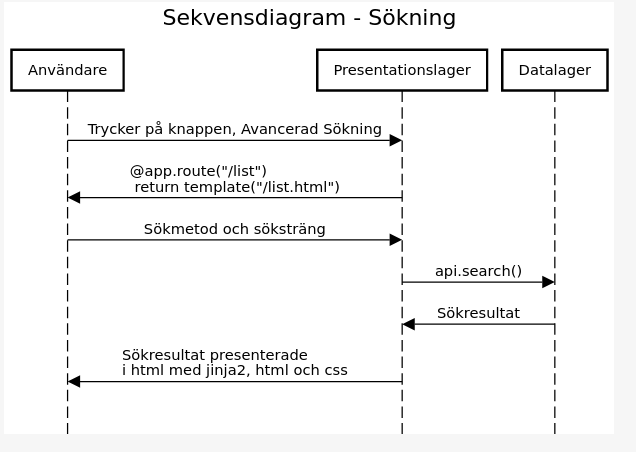
\includegraphics[width=\textwidth, height=10cm]{/home/danhu849/tdp003/Pictures/Sekvensdiagram.png}}
  \caption{Sekvensdiagram för Sökning \label{fig:1}}
\end{figure}

I sekvensdiagram \ref{fig:1} visas det översiktligt hur användaren från (/home, /) presenteras med sökresultat.

\section{Felhantering och Loggar}
Samtliga portfoliohändelser loggas med hjälp av Pythons logging.config modul. Konfigurationen för loggningen definieras i filen <logging.cfg>. Loggar skrevs till filen <portfolio\_log.log> i kronologisk ordning. Senast log längst ner. Båda filerna finns i root katalogen för portfolio-appen. Loggar sparas med datumstämpel, viktighet, namn, tråd och meddelande. Alla loggar skrivs in i logfilen oavsett viktighet, men kan ändras vid behov genom att ändra <level=DEBUG> under <[logger\_root]> i konfigurationsfilen <logging.cfg>. En nivå som filtrerar bort mer än DEBUG rekommenderas ej då händelser som lett upp till kraschen kan ha filtrerats bort. Logfilen finns tillgänglig även när flask inte körs. Vid ny körning av flask skrivs inte portfolio\_log.log över utan nya loggar skrivs in längst ner i filen.

Terminalkommandot tail med flaggan -f används vid flask run för att i realtid övervaka de senast tillagda loggarna i <portfolio\_log.log>. Vid behov används flaggan -nN där N definieras av antalet rader som visas. Utan flaggan -n visas de sista 10 raderna från filen i terminalen. Att alltid de 10 sista raderna visas från filen möjliggörs av flaggan -f.

<code>tail -n15 -f /path/to/portfolio\_app/portfolio\_log.log</code>

Utöver logfilen hanteras fel med hjälp av pythons print() funktion som kan skrivas in i varje @app.route() funktion, men också egendefinierade funktioner. Informationen skrivs ut i terminalfönstret när funktioner aktiveras under en flask run körning. Med print() kan variabler från bland annat databasen kommas åt. Flasks egen debug mode aktiveras genom att FLASK\_DEBUG variabeln sätts till 1 innan flask run:

<code>export FLASK\_DEBUG=1</code>

\subsection{Testning/felsökning - Databas}
Testning av datalagrets funktioner tillhandahålls av kursledningen och benämns enhetstester. Utöver de initiella enhetstesterna har fler med tiden lagts till. Enhetstesterna skrevs i python3 där pythons modul unittest (Unit testing framework) används. Testerna skrevs med kravspecifikationen i åtanke. Körning av testerna utan fel bevisar att funktionens krav uppfylls. Funktionerna för datalagret felsöks lättast med print() funktionen.


\end{document}
